\documentclass[tikz,border=10pt]{standalone}
% No extra TikZ libraries needed: all coordinates are precomputed.
\begin{document}
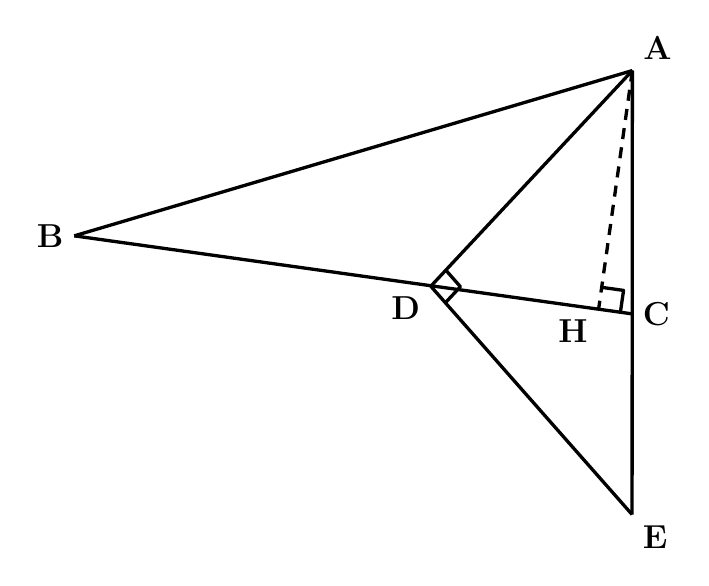
\begin{tikzpicture}[line width=1.2pt, line join=round, font=\fontsize{12}{14.4}\selectfont]
  % Named points (scale s = 0.014981 cm/px, y flipped, centred on ink bbox)
  \coordinate (A) at (3.540,2.818);
  \coordinate (B) at (-3.547,0.719);
  \coordinate (C) at (3.536,-0.272);
  \coordinate (D) at (0.980,0.079);
  \coordinate (E) at (3.536,-2.820);
  \coordinate (H) at (3.111,-0.212);

  % Solid segments
  \draw (B) -- (A);
  \draw (B) -- (C);   % passes through D
  \draw (A) -- (D);
  \draw (D) -- (E);
  \draw (A) -- (E);   % passes through C

  % Dashed segment A-H
  \draw[dash pattern=on 4pt off 3pt] (A) -- (H);

  % Right-angle mark at H (between HA and HC)
  \draw (3.151,0.065) -- (3.428,0.026) -- (3.388,-0.251);

  % Right-angle mark at D (between DA and DE)
  \draw (1.171,0.283) -- (1.356,0.073) -- (1.165,-0.131);

  % Labels (bold math to match original weight; vertex dots removed)
  \node[above right] at (A) {$\mathbf{A}$};
  \node[left] at (B) {$\mathbf{B}$};
  \node[right] at (C) {$\mathbf{C}$};
  \node[below left] at (D) {$\mathbf{D}$};
  \node[below right] at (E) {$\mathbf{E}$};
  \node[below left] at (H) {$\mathbf{H}$};
\end{tikzpicture}
\end{document}